\documentclass{article}
\usepackage{xeCJK}
\setCJKmainfont{MS Mincho} % for \rmfamily
\setCJKsansfont{MS Gothic} % for \sffamily
\author{Richard Gendal Brown, James Carlyle, Ian Grigg, Mike Hearn}
\date{2016年8月}
\title{Corda:  イントロダクション}
%%\setlength{\parskip}{\baselineskip}
\usepackage{amsfonts}
\usepackage{listings}
\usepackage{color}
\usepackage{epigraph}
\usepackage{graphicx}
\graphicspath{ {images/} }
\usepackage[export]{adjustbox}
\usepackage{float}
\usepackage{hyperref}
\usepackage[super,comma,sort&compress]{natbib}
\usepackage[nottoc]{tocbibind}
%\usepackage[natbibapa]{apacite}
\renewcommand{\thefootnote}{\alph{footnote}}
%\epigraphfontsize{\small\itshape}
\setlength\epigraphwidth{4.5cm}
\setlength\epigraphrule{0pt}
\begin{document}
\maketitle
\begin{abstract}
相互に信頼しないノードが共有する分散台帳により、金融機関や個人間における取引や債務を記録する、ひとつのグローバルデータベースが可能となるでしょう。現在、別々に管理されている台帳を同期するために実施している手作業の多くは削減されるでしょう。また、今よりもより多くのコードが共有され、金融サービスのコスト削減につながるでしょう。私たちは、これらの目標を達成するために設計したCordaをここに発表します。このペーパーでは、一般の読者向けに概要レベルのイントロダクションを提供します。続けて公表されるテクニカルホワイトペーパーにて、設計とCordaアーキテクチャー採用の背景を詳細します。
\end{abstract}
\newpage
\tableofcontents
\newpage
\section{イントロダクション}
R3は、分散台帳技術が金融業界を変革し、顧客や関係者に便益をもたらす可能性を秘めていると考えています。私たちは金融取引が自動でエラーなく記録・管理され、誰もがシームレスにどんな契約でも取引出来るようになる未来を思い描いています。金融取引の当事者が取引を記録し、共有し、協働で正確に台帳をメンテナンスするやり方に変わっていくと考えています。重複やリコンシリエーション、認識相違等は過去のものとなるでしょう。各社が別々に資産を記録することもなくなっていくでしょう。
私たちは、信頼できるテクノロジーを活用することで、既存の法的枠組みの中で展開できる金融のユースケース向けに共有台帳を定義しようとしています。私たちの考えは三つのカテゴリーに細分化できます。金融機関の要件の実装、非機能要件へのフォーカス、そして拡張性です。
このペーパーでは、私たちが規制された金融機関向けに最適だと考えるCordaプラットフォームの設計上の特徴について紹介させて頂きます。\footnote{著者のメールアドレス: Richard Gendal Brown \href{mailto:richard@r3cev.com}{(richard@r3cev.com)}, James Carlyle \href{mailto:james@r3cev.com}{(james@r3cev.com)}, Ian Grigg \href{mailto:iang@r3cev.com}{(iang@r3cev.com)}, Mike Hearn \href{mailto:mike@r3cev.com}{(mike@r3cev.com)}}
\section{背景}
銀行は世の中で思われいるよりも早くから情報技術を受け入れ、手作業の自動化、処理のデジタル化を成功させてきました。しかしながら今、そのコストと効率性を著しく向上させるアーキテクチャーが登場してきています。
各金融機関は独自の台帳を維持しており、顧客や相手方との契約やポジションについてその会社目線での見え方を記録しています。一方、相手方は相手方の見え方で取引を記録しています。この重複作業が不一致を引き起こし、取引に関連する様々な当事者間でマッチング、リコンシリエーション、エラーの修正を必要とさせるのです。同じトランザクションに対する見え方の違いの程度によっては、潜在的にシステミックな危険を孕んでいるとも言えます。
複数の金融機関で競争することは良いですが、複数のテクノロジーで複雑さとオペレーションリスクを増加させてしまうことは良くありません。しかしながら、近年までこれは避けられませんでした。中央集権型の市場インフラを除いて\footnote{例としてDepository Trust \& Clearing Corporation (DTCC)やContinuous Linked Settlement Group (CLS).}, 、企業間のテクノロジーを統合する良い方法は(会社の合併なしで)ほとんどありませんでした。 
中央集権型の市場インフラユーティリティーはデータ量の増加と企業間でのビジネスロジックの共有という観点である程度上手く行きました。しかし、webの登場以来、情報技術の分野で達成してきたレベルに比べ、金融取引分野で統合はまだ遅れを取っています。\cite{IT}

私たちは、暗号化技術の成熟や、いわゆる”ブロックチェーン技術”に代表される技術が、新たな機会を提供すると考えています。すなわち、企業間で安全にレコードを共有するシステムの可能性です。このビジョンは金融機関の経済を変革するかもしれません。金融イベントの記録やビジネスロジックの処理のために、新たな共有プラットフォームを実装することで、(これだけではないですが)特にポストトレード分野における変革をもたらします。企業間における全ての取引が信頼できる唯一でグローバル論理台帳に記録するのです。このアーキテクチャーは業界の新たな共有プラットフォームを定義し、この上で、現行の金融機関、新規参入者、第三者機関が競合し、革新的な商品やサービスを展開することができます。
\begin{figure}[H]
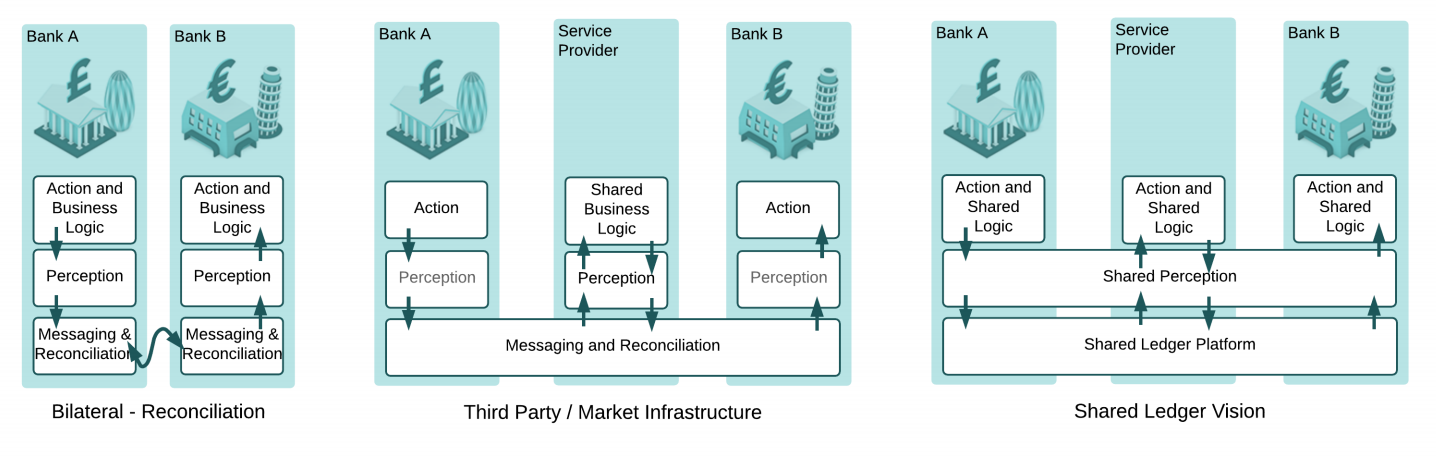
\includegraphics[scale=.5, center]{sharedlogic}
\caption{上記の図は、不一致や重複がありながらも共有する事実を独自に記録・管理している世界(\textit{``リコンサイルを除いた相対取引"})もしくは中央集権型ユーティリティーに権限と責任を委譲する世界(\textit{``第三者/市場インフラ"}), から、協働で共有レコードを維持し、一貫性を確保し、既存/新規事業者および市場インフラ事業者がオープンに競争し、サービスを利用する世界(\textit{``共有台帳ビジョン"}).への進化を表しています。}
\end{figure}
私たちは、高品質なデータが企業間で不一致を減らし、迅速に合意形成をする上で重要になると考えています。さらに、企業を跨ぐこの共通アーキテクチャーの実装により、新たなプラットフォームが定義され、既存および新規事業者は顧客ニーズに合ったサービスを提供するために、競合することになるでしょう。また、企業内では複数のシステムに同じ取引を記録するという課題がコストと複雑化を助長する要因となっていますが、これを解決するアプリケーションも出てくるでしょう。
\section{ビジョン}
長期的には、全ての経済主体が相互にやり取り出来る、``グローバル論理台帳" を思い描くことが出来ます。誰でも安全で一貫性があり、信頼できてプライバシーも確保された方法で取引を記録・管理することが可能となります。グローバルと呼んでいるのは、誰でも取引相手と同じデータを見ることが出来るという意味で、論理と呼んでいるのは、物理的な実装は企業によって異なってくるという意味です。将来像は、企業内で維持される記録システムから、\textit{企業間}で共有されるグローバルな記録システムとなるでしょう。
\subsection{将来像を支える考え方}
分散台帳技術を活用した将来像を支える基本的な考え方は以下となるでしょう。
\begin{itemize}
	\item 契約に従い台帳に記録される事実には、紛争時に適用出来る法的根拠が与えられる。
	\item 台帳に記録される事実は、他の場所で保持されるマスターデータのコピーという位置付けよりも、むしろ権威あるものとして認識される。これにより、プラットフォーム間での決済は直に行われる。
	\item 一度取引当事者が合意すれば、台帳上の事実はファイナリティーを与えられ、改ざん不可となる。エラーや巻き戻しは後続のトランザクションを通じて行われる。企業は内部プロセスの正確さと品質向上に向けた見直しを迫られる。
	\item 信頼のある主体は、原則として、直接台帳に接続し、相手方との取引を記録する。相対取引を強制する訳ではないが、”重層化”もしくは階層化した市場モデルは少なくなるかもしれない。
	\item オープンスタンダートを推進することで、既存および新規事業者が協業・競合し、差別化したサービスを提供することで、より多くの選択肢をもたらす。
	\item 取引の内容を知る必要のある範囲の当事者だけが、当該金融取引にアクセスすべき正当な権限を持つ。
\end{itemize}
しかしながら、このビジョンは道半ばの状況を型取っており、まずはビジネスロジックの共有に専念するかもしれません。これは、今日私たちが使用しているシステムと当面の間共存する必要があるためです。統合や移行はソリューション設計上、重要な部分であると認識しています。道半ばではあるものの、長期的ビジョンのうち、リーガル面および他のテクニカル以外の部分を同時並行で取り組むことは、それだけでも大きな価値をもたらすでしょう。
グローバル論理台帳という方向性を示しつつも、それが複数の台帳により実現される可能性がある点について今一度強調しておきたいと思います。おそらくこれは、アセットクラスごとに一つの台帳の形となるか、自発的に緩く結びついて、異なるビジネスサービス間で独立した機能・運営となるかもしれません。

このビジョンを支えるアーキテクチャー上の戦略的な判断は以下になります。
\begin{itemize}
\item このシステムにより管理されるレコードは、資産や取引に対し正当な権利を持つ者だけがアクセス可能となる。
\item 取引の挙動はシステムにより管理され、コンピューターコードにより表現される。コンピューターコードの正当性は参照する法律文書により確保する。\cite{Ricardian}
\item コントラクトコード更新のサポート。紛争解決の手続きが成立しない契約をどう進めれば良いかをサポートする。これは、いくら自動化しても、契約上の紛争は発生し、結果としてテクニカルと人手の両方を必要とすることになるためである。
\item このビジョンが実現すれば、コスト、リスクや規制対応負荷(資本、流動性およびオペレーション上の義務)が軽減され、新たな商品やサービスの開発に繋がる。
\item 金融業界に広く普及するために、システムの一部はオープンにすべき。すなわち、オープンソース、オープンな開発プロセス、オープンスタンダードであること。
\item このビジョンは”プラットフォーム”もしくは”システム”の観点で語られているが、事業者が競合・協業し、異なるレイヤーで異なる商品・サービスを実現出来るようになる考えている。垂直統合により我々が独占してしまうようなアプローチは思い描いていない。
\item このビジョンはまた、一番上位のレイヤーで個別の企業やグループが独自のIPを保持することを想定している。
\item このシステムはセキュリティが確保された環境の下で運営する。高まるサイバー犯罪の脅威は所与のものとして考慮されるべき。
\end{itemize}
このビジョンの実現に必要な基本技術は既に存在すると信じられていました。これらには(これだけに限りませんが)、暗号化技術、グローバルコミュニケーションネットワーク、金融商品の標準化や本格的な運営にも耐え得るアルゴリズムを含みます。
このビジョンを可能とするものは、近年における分散台帳およびブロックチェーンへの関心の高まりです。このようなビジョンがオープンに議論され、複数の金融機関の協働を通じて、環境が整ってきました。ネットワークの参加者間でのIDインフラの構築が想定されていますが、具体的にどうオペレーションが改善されるかまでは想定を置いていません。当局の巻き込みがプロセス設計上の鍵となります。
私たちは、金融機関の要件と既存の分散台帳プラットフォームを評価した結果、既存のプラットフォームでは、金融機関のニーズに対応出来ないとの結論に達しました。つまり、これまでの分散データベースの設計を支えるスレッドモデルは、相互に信頼しない法人格が合意に至るためのユースケースには合いませんでした。既存のブロックチェーンのアーキテクチャーは、個別の契約レベルで特定のデータを制限しシェアするという要件には合わないのです。その結果、私たちはCordaを設計・開発致しました。
\section{Corda}
Cordaは金融取引を記録・処理するための分散台帳プラットフォームであり、このドキュメントに記載しているビジョンを実装するために設計されました。
Cordaは、Clack, Bakshi, Braineが定義するスマートコントラクトをサポートします。\cite{SCT} 私たちのスマートコントラクトでは、人による入力をもとに、コンピューターコードがその実行を自動化します。債権や債務は法律文書で表現されるように、法的に執行力を持ちます。スマートコントラクトは法律文書に関連したビジネスロジックとデータにリンクし、プラットフォーム上の金融取引に法的執行力を持たせ、曖昧さや不確実性、紛争時における明確な拠り所とすることが出来ます。
\subsection{基本的な特徴}
Cordaは規制されている金融機関向けの利用に特化しています。ブロックチェーンに大きく影響されていますが、多くの金融向けシナリオには不適切なブロックチェーンは採用しませんでした。
Cordaはスマートコントラクトを実行するフレームワークであり、以下の特徴を持ちます。
\begin{itemize}
    	\item{金融取引の遷移を記録・管理し、既存の法的枠組みの中で二者以上の当事者間で共有するデータが根付く土壌となり、既存および今後課される規制にも対応}
	\item{中央集権型管理者なしで企業間におけるワークフローの振る舞いを管理}
	\item{グローバルな台帳レベルではなく、個別取引レベルで合意形成をサポート}
	\item{当局による監督者ノードをサポート}
	\item{トランザクションの検証は当事者間だけで実施}
	\item{様々なコンセンサスメカニズムをサポート}
	\item{人が理解できる法律文書とスマートコントラクトのコードとの明確なリンクを記録}
	\item{業界標準のツールを使用}
	\item{資格を有する者もしくは正当な権限を持つ者だけに取引データへのアクセスを制限}
\end{itemize}
これらの特徴が、複雑な金融機関での利用に適したプラットフォームの設計に貢献しています。この設計では、ネイティブな仮想通貨を使ったりやグローバルなトランザクションの速度制限を課したりしません。
\subsection{コンセプト}
私たちは、信頼できる唯一のデータソースであるグローバル台帳という考え方から始めました。しかしながら、トランザクションと台帳への記帳をグローバルに見える化してしまうことは私たちのモデルには合いませんでした。トランザクションは当事者による小グループ内だけに留め、関連データはグループ内だけで維持出来るようにしたかったのです。
私たちのコンセプトにおける一番基本的な概念は\textit{ステートオブジェクト}と言います。これは電子的ドキュメントであり、二者以上の当事者間における合意の存在、内容、現状のステータスを記録します。ステートオブジェクトは、参照する正当な理由を持った者だけの間で共有されます。全ての参加者に全てのデータが参照可能となっていない共有システムにおいて、グローバルで一貫性を保つために、私たちは当事者とデータを特定するために暗号化技術(ハッシュ)を活用しています。台帳は改ざん不能なステートオブジェクトの集まりとして定義されます。
私たちは合意のステートオブジェクトという観点で考えていますが、目的はこのステートオブジェクトが遷移する度に、取引に関係する全当事者が合意形成することです。これはブロックチェーンのコンセプトだと言う人もいるかも知れませんが、単純な支払処理から複雑なスマートコントラクトの処理に至るまで、異なる主体により保持されるデータが、更新されても一貫性を保つことで、信頼できる取引基盤を形成することが出来るのです。
\begin{figure}[H]
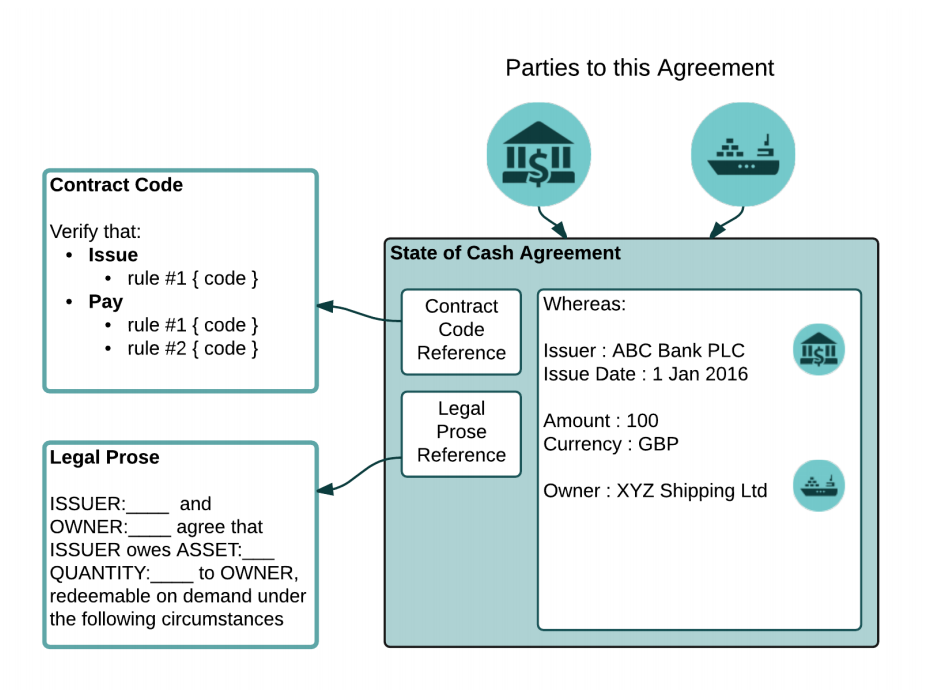
\includegraphics[scale = .4, center]{partiesto}
\caption{上記図では、ステートオブジェクトが商業銀行に対する100ポンドのキャッシュ請求権を表しています。キャッシュのオーナーは架空の船会社です。このステートオブジェクトは取引を管理する法律文書とその遷移を管理するコントラクトコードへのリンク(ハッシュ)を持っています。}\end{figure}
参加者が台帳全体の状態もしくは仮想マシン全体でコンセンサスを取るシステムとは対照的に、私たちは合意のステートオブジェクトにフォーカスしています。Cordaはグローバルで分散された合意形成を実現するために、以下3つのツールを提供します。
\begin{itemize}
    \item 事前に合意したルールに則り、ステートオブジェクトの遷移が有効であるかを検証するスマートコントラクトのロジック
    \item トランザクションを一時的に並べて衝突を回避するユニークネス(一意性)およびタイムスタンプサービス
    \item 複数の異なる当事者間で、何ステップもの複雑なやり取りを書くプロセスを単純化するオーケストラフレームワーク
 \end{itemize}
\subsection{コンセンサス}
Cordaでは、\textit{トランザクション}を使って更新が行われます。既に存在するステートオブジェクトを消費し、新しいステートオブジェクトを生成します。ここで二つ合意形成がなされます。
\begin{enumerate}
\item{トランザクションの妥当性:アウトプットのステートオブジェクトを定義する更新トランザクション(提案された状態)が有効であること、関連するコントラクトコードが問題なく実行され必要な署名がされていること、このトランザクションを参照する全てのトランザクションもまた有効であること、以上により、当事者は取引に確信を持ちます。}
\item{トランザクションの一意性:インプットとなる全てのステートオブジェクトがそのトランザクションだけで消費されること、すなわち、同じステートオブジェクトを消費する他のトランザクションが過去に存在しないこと、これにより当事者は取引に確信を持ちます。}
\end{enumerate}
当事者は、別々に同じコントラクトコードとバリデーションロジックを走らせることで、トランザクションの妥当性に合意することができます。しかしながら、一意性に対するコンセンサスには事前に決めておいたオブザーバーが必要となります。多くの場合、独立したノードになるかと思います。
\begin{figure}[H]
    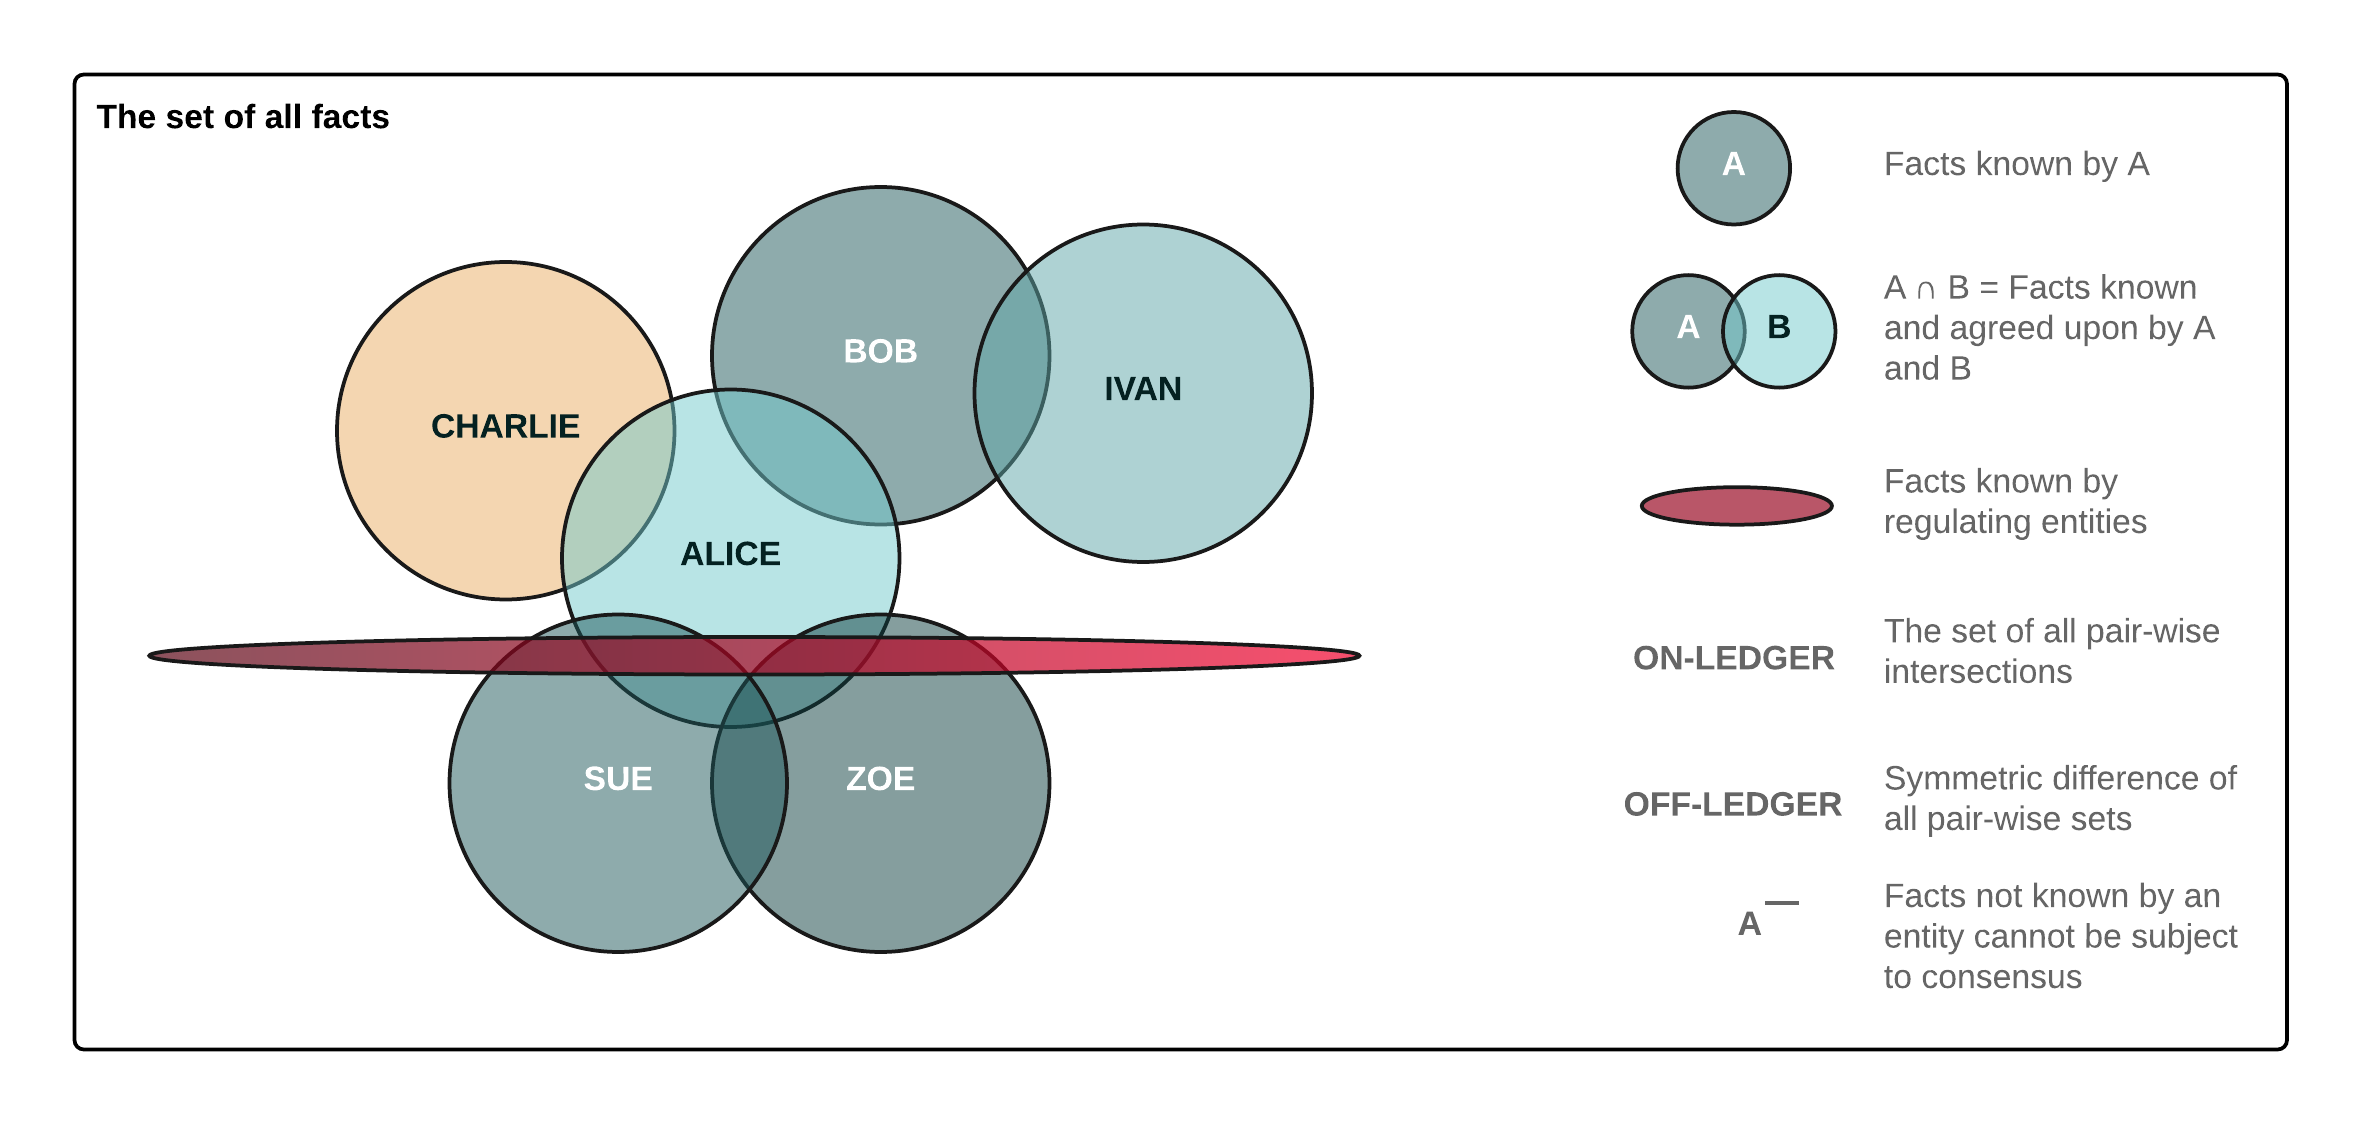
\includegraphics[scale = .5, center]{Consensus}
    \caption{トランザクションの妥当性に対するコンセンサスは、そのトランザクションに関する当事者だけにより検証されます。そのため、データはそれを見る必要のある人だけに配信されます。他のプラットフォームでは、一般的に台帳レベルでコンセンサスを取ります。Cordaでは、システム全体として管理しているデータの一部分だけが当事者に共有されます。少なくとも二つの主体がデータの存在と詳細についてコンセンサスに至っているのであれば、それは``on-ledger"と言えます。Cordaでは、任意の主体の組み合わせで、あらゆるデータの合意形成プロセスを実施することが可能です。データが一つの主体により保持されている場合、``off-ledger"と言えます。}
\end{figure}
Cordaのユニークネスサービスは``追加可能"です。これにより、プライバシー、スケーラビリティー、リーガルシステムとの互換性\cite{EUC} やアルゴリズムを強化することができます。あるサービスはビザンティンフォールトトレランスアルゴリズムによって、相互に信頼しない多数のノードにより構成されるかもしれません。もしくはスタンドアローンのようにシンプルな作りになるかもしれません。ある場合は、ステートオブジェクトの遷移に全ての当事者の署名が必要となるかもしれません。その場合、ユニークネスサービスは全く必要なくなるでしょう。
重要な点は、これらユニークネスサービスが、ステートオブジェクトがトランザクションにより事前に消費されているかどうかを検証するためだけに必要であるという点です。トランザクションそのものを検証するために必要なのではありません。それはトランザクションに関係する当事者間の問題となります。つまり、ユニークネスサービスはトランザクションの中身まで見る必要はないということです(また、見せるべきでもありません)。これにより、他の分散台帳やブロックチェーンに比べて、プライバシーとスケーラビリティーを著しく向上させています。この設計上の判断は、共有台帳アーキテクチャーにおけるトレードオフについて重大な影響を及ぼしています。今後発表するテクニカルホワイトペーパーの中で詳細は議論したいと思います。
\subsection{ビジネスロジック}
Cordaはスマートコントラクトのコードを通じてビジネスロジックを実行します。スマートコントラクトは、取引を受け入れるか拒否するかの機能を提供し、シンプルで再利用可能な機能で構成されています。トランザクションを解釈し、インプットとしてステートオブジェクトを受け取り、アプリケーションのコマンド(スマートコントラクト)によりアウトプットのステートオブジェクトを生成します。提案されたアクションが有効であれば、トランザクションは受け入れられます。コントラクトコードはビジネスロジックを定義し、また可動性があります。規制のある場面では署名したコードを使う想定ですが、ノードはデプロイ時にチェックなしで、サンドボックスの中のコントラクトコードをダウンロード・実行します。
コントラクトコードの実行と検証のために、私たちはJava Virtual Machine\cite{JVM}を選択しました。既存のライブラリーが豊富で、スキルを持った開発者が多数いるからです。業界標準のツールを使うことで、銀行は既存のコードを簡単に再利用することができます。しかし、通常のJVMよりもより制限を厳しくしたカスタムサンドボックスを使うことで、セキュリティー要件だけでなく、確定的な実行環境を提供しています。イーサリアム6のように、バイトコードを標準化する選択肢が用意しており、ユーザーは好みによって、コントラクトコードの言語を変えたり、もしくはよく知られている言語を再利用することが出来ます。内部アプリケーションから直接コントラクトコードを利用することも簡単です。一度コントラクトコードがレビューされていれば、アプリケーションの開発はかなりシンプルなものになるでしょう。
\subsection{コアとなる金融コンセプト}
Cordaのアーキテクチャーは3つの設計上鍵となるユースケースにより強く影響されています。これらは解決すべき共通の課題を内包していると考えられています。そのユースケースとは、キャッシュ、証券化商品、そしてデリバティブ取引です。
\begin{itemize}
\item キャッシュの残高(例えば、``私は、百万ドルを預けていることを銀行と同意している")
\item 預託している証券化商品(例えば、``私は、この会社の株を1,000株保有していることを銀行と同意している")
\item 相対デリバティブ取引(例えば、``銀行Aと銀行Bは次の金利スワップに同意している。すなわち、次のキャッシュフロー(ネット)を事前に取り決めしたスケジュール、支払条件に従って交換すること。")
\end{itemize}
ここでは一つ例を取り上げます。Cordaのキャッシュの設計は”銀行の中にお金”のようなものは存在しないという現実をモデリングしており、銀行に対しキャッシュの請求権を所有者が持っているだけです。\cite{BOE}つまり、私たちの考えるキャッシュの契約はシンプルですがとても有用です。キャッシュ発行者である法人、通貨、金額、所有者を記録し(その他請求権の特徴を考慮した他の情報、またこの合意を管理する\textit{法律文書}への明確なリンクを付します。これは紛争時の解決手段として使用されることを想定しています)、これらはその他キャッシュ関連のコンセプト(支払、ネッティング等々)を構築する際に使用されます。
\begin{figure}[H]

\includegraphics[scale = .4, center]{cash}
\caption{上記は、最もシンプルなCordaのトランザクション(キャッシュの発行)を示しています。商業銀行から架空の船会社に、新しいキャッシュのステートオブジェクトが発行されているのが分かります。この発行のトランザクションは発行銀行により署名されます。このようなシンプルなモデルから、支払、DVP決済や先日付の債務のような複雑なトランザクションに至るまで構築が可能です。}
\end{figure}
\subsection{Cordaモデルのまとめ}
私たちのモデルにおけるコアコンセプトは以下の通りです。
\begin{itemize}
\item \textit{ステートオブジェクト}, 二者以上の当事者間における合意を表し、機械が読み込める\textit{コントラクトコード}により管理されます。そしてコントラクトコードは人間が読み込める\textit{法律文書}を参照し、実装されるものです。
\item \textit{トランザクション}, ステートオブジェクトを遷移させていきます。
\item \textit{トランザクションプロトコル}または\textit{ビジネスフロー}, 中央管理者なしで、取引の当事者が次のアクションを調整することを可能とします。\end{itemize}
プログラミングのテクニックによりステートオブジェクトの共有を最小限の範囲に留めつつ、取引の確定を実現します。
ステートオブジェクト(データ)、コントラクトコード(許容するオペレーション)、トランザクションプロトコル(ビジネスロジックの振る舞い)、その他必要なAPI、ウォレットプラグインやUIコンポーネントの組み合わせにより、共有台帳アプリケーション、もしくはCorda分散アプリケーション(\textit{``CorDapp"})は構成されます。これは開発者がプラットフォーム上で作ることとなる、コンポーネントのセットになります。
%\begin{figure}[H!]
%\includegraphics[scale = .4, center]{image4}
%\caption{Current thinking on the applications in the Corda-driven ecosystem.}
%\label{fig:figure4}
%\end{figure}
%\begin{figure}[H!]
%\includegraphics[scale = .25, center]{image5}
%\caption{Another visual representation on how Corda will interact with the financial ecosystem.}
%\label{fig:figure5}
%\end{figure}
\section{他プラットフォームとの比較}
Cordaは金融機関の実務担当者の協力により制作され、金融機関の要件に基づき設計されました。しかしながら、そのデザインはTodd Boyle と Ian Grigg による triple entry accounting\cite{Triple}やBitcoin\cite{Bitcoin}やイーサリアムのような既存の分散台帳プラットフォームにもインスパイアされています。そのため、これらのプラットフォームとの関係においてCordaを理解した方が分かりやすいかもしれません。
\subsection{ビットコインとの比較}
Cordaはビットコインと非常に似ている部分があります。
\begin{itemize}
\item{トランザクションにより生成・消費される改ざん不能なステートオブジェクト。}
\item{トランザクションは複数のインプットとアウトプットを持っています。ビットコインは未使用トランザクションアウトプット(UTXO)として台帳を参照します。}
\item{コントラクトコードは単なる機能です。ストレージは持っていませんし、他とやり取りすることも出来ません。同じトランザクションを想定すると、コントラクトコードの”検証”機能は常に同じ結果を出力します。}
\end{itemize}
しかしながら、ビットコインのトランザクションは単一で固定したデータフォーマットであり、ビットコインの量と関連するルール(スクリプト)以外のデータを保持することはほぼ出来ません。コントラクトコードのカスタマイズ可能な箇所にデータを組み込むことで、この制限を回避しようとする試みもあります。パターンマッチングを通じてデータを抜き取ることが出来ますが、これは良いアプローチとは言えません。これに対し、ステートオブジェクトは任意のデータタイプを扱うことができます。加えて、トランザクションはインプットとなるコントラクトだけでなく、アウトプットとなるコントラクトも起動できます。ビットコインのトランザクションは、消費されたインプットのステートの中のコントラクトコードによりコントロールされます。私たちが呼ぶ”コントラクト”という用語は、トランザクションの検証以上に、多彩なタスクをハンドリング出来るビジネスロジックのことを指しています。例えば、現在、私たちのコントラクトもまた有効なトランザクションを生成するコードを含んでいます。(これはビットコインの”ウォレットコード”に当たります)
ビットコインのスクリプトはインプットとして、固定のバイト配列を受け取ります。これは、コントラクトがトランザクション全体の構造を精査する他の方法がないことを意味しており、コントラクトに制限を課しています。私たちのコントラクトはチューリング完全であり、JVM上で動く普通のプログラミング言語で書かれています。Cordaは、ブロックがマイニングする時間に左右されず、任意の時間に正確にトランザクションを実行することが可能です(信頼できるタイムスタンパーによる認証が必要)。私たちがサポートする多くの契約が正確なタイミングを必要としていることを考えると、私たちの合意形成の方式である、ブロックを使わずに衝突を解決するアルゴリズムは重要となります。Cordaは、プルーフ・オブ・ワークを利用せず、``マイニング"のコンセプトも持っていないのです。
\subsection{イーサリアムとの比較}
イーサリアムでは、コードは仮想マシンの中で実行され、複雑なロジックを実装可能です。コントラクトのプログラミングには、ノンアセンブリベースの言語が使用されます。様々な種類の金融取引のモデリングを想定しています。
しかしながら、イーサリアムにおける``コントラクト"という用語は、全ての参加者ノードによりメンテされ、複製されるプログラムの初期化を意味します。この初期化はオブジェクト指向言語のオブジェクトのようなものです。メッセージを送受信したり、ローカルのストレージを更新したり出来ます。一方、私たちのスマートコントラクトの実装は一連の機能を意味しており、そのうちの一つがシステムを同期させる機能になります(\textit{検証機能})。この機能は全くのステートレスです(すなわち、実行中に他システムとやり取りしません)。コントラクトコードは可変のストレージを持っていないため、``メッセージ"という考え方はありません。イーサリアムは金融のロジックだけでなく、文字通りどんなアプリケーションにも対応するプラットフォームであると主張しています。私たちのプラットフォームは、少なくとも最初は非金融向けアプリケーションをスコープ外としております。

%\section{Worked Example: Cash}
%A state object (depicted ) represents an agreement shared between parties.

%States contain arbitrary data, but they always contain at least a reference to the hash of a contract code, which is a program expressed in some byte code that runs sandboxed inside a virtual machine, and a reference to the hash of a legal prose document, which provides legal context in a form that is recognised by a judicial or other dispute resolution system. \textit{Contract code} (or just “Contracts” in the rest of this document) are globally shared pieces of business logic. Contracts always define a verify function, which is a pure function that is able to determine whether the transition for the State is valid, regardless of which party calls the function. The verify function does not check that a transaction is in the interests of either party, only that its constraints are enforced, and nodes must separately satisfy themselves the transaction is in their own interests. This is discussed more later.

%In the diagram above, we see a stylised \textit{cash state object}, which represents the ownership of 100 USD. The object refers to its governing contract and associated legal prose. As this is a cash contract, the legal prose document will specify the terms and conditions that pertain to a cash liability issued by one party to another: under what circumstances can the cash object be redeemed for a balance in a traditional bank account or in exchange for a wire transfer elsewhere? How will disputes be resolved? And so forth. In addition, the legal prose will specify those rights, obligations and conditions associated with the contract which the parties agree will be automated through computer code. We will explicitly delegate from the legal prose domain to the code domain.

%Furthermore, and critically, the legal prose will also leave several pieces of information unspecified: who is the issuer and what is the currency? The state object contains these fields (we see the issuer here is Barclays Bank PLC and the currency is USD).The combination of the legal prose, contract code and parameters captured in the state object plus relevant digital signatures collectively define the agreement between the parties.

%In what follows, we describe how an instance of a state object, such as the one above, can be evolved, processed and transferred between parties using the other components of the Corda architecture.

%Note: At a very high level, this design is analogous to a "UTXO model" such as bitcoin's. However, it also has some significant differences. The choice of a UTXO-style model rather than an account/balance model such as that used in Ethereum is a conscious and deliberate choice and is foundational to the privacy and scalability characteristics of the platform

\section{ロードマップ}
現在の設計思想に辿り着くまで、私たちは当初Cordaのプロトタイプを開発し、シミュレーションして、コンセプトを検証しました。網羅的ではありませんが、短中期的に実装しようとしているCordaの追加機能を以下に示します。
\begin{itemize}	
\item トランザクションの分割と一意性の向上:ユニークネスサービスからの読み込みを困難とするトランザクションの部分的な不可視化メカニズムの取り込み
\item コントラクト検証サンドボックス:コントラクト実行のための最小限Javaライブラリーセットのホワイトリスト
\item 残高等ポジション計算のためのプラグインベースウォレット
\item 参加者が利用できる特定ビジネスロジックへのゲートウェイやオラクル(仲介ノードや評価エンジン等)
\item ユーザーのID管理が出来るCordaモデルの利用
\item 相互運用可能性とデータ統合、特にFpML, ISO20022。他データフォーマットや他プラットフォームとの統合/相互運用可能性のサポート
\item レファレンスデータのためのアプリケーション構築
\item アドレスのランダム化、ゼロ知識証明、資産再発行スキームなどの技術を使ったプライバシーの向上
\item より多くの金融商品の実装
\item ステートオブジェクトの集約など、ポートフォリオレベルのビジネスロジックのサポート
\end{itemize}
\section{結論}
今日における既存の分散台帳とブロックチェーン技術とは異なり、Cordaは金融機関における取引の記録・執行という明確な目的のために開発されました。汎用的なソリューションで、全ての課題を解決しようとしている訳ではありません。そのため、データ配信とトランザクションセマンティクスに独自のアプローチを採用しております。一方で、金融機関にとって魅力的な分散台帳の特徴も維持しています。すなわち、金融取引を自動でかつ実効性のある方法で実行するという特徴です。
\bibliographystyle{unsrt}
\bibliography{Ref}
\end{document}